\documentclass{osa-article}
\journal{none}
% \articletype{Research Article}

\usepackage{lineno}
\linenumbers

\begin{document}

\title{Summary of Meshtalk}

\author{Jay,\authormark{1}}

\address{
  \authormark{1}Jay from CAU EAI Lab
  }

\email{\authormark{*}woong712@cau.ac.kr} %% email address is required

\homepage{https://yukinyaa.github.io} %% author's URL, if desired

%%%%%%%%%%%%%%%%%%% abstract %%%%%%%%%%%%%%%%
%% [use \begin{abstract*}...\end{abstract*} if exempt from copyright]

\begin{abstract}
\LaTeX{} Meshtalk is a generic method for generating full facial mesh animation from speech. It can generate 'lipsync' animation from a single frame of generic human facial mesh, and also can mix in emotional information from mesh animation.
\end{abstract}

%%%%%%%%%%%%%%%%%%%%%%%%%%  body  %%%%%%%%%%%%%%%%%%%%%%%%%%
\section{Introduction}
\begin{figure}[h!]
\centering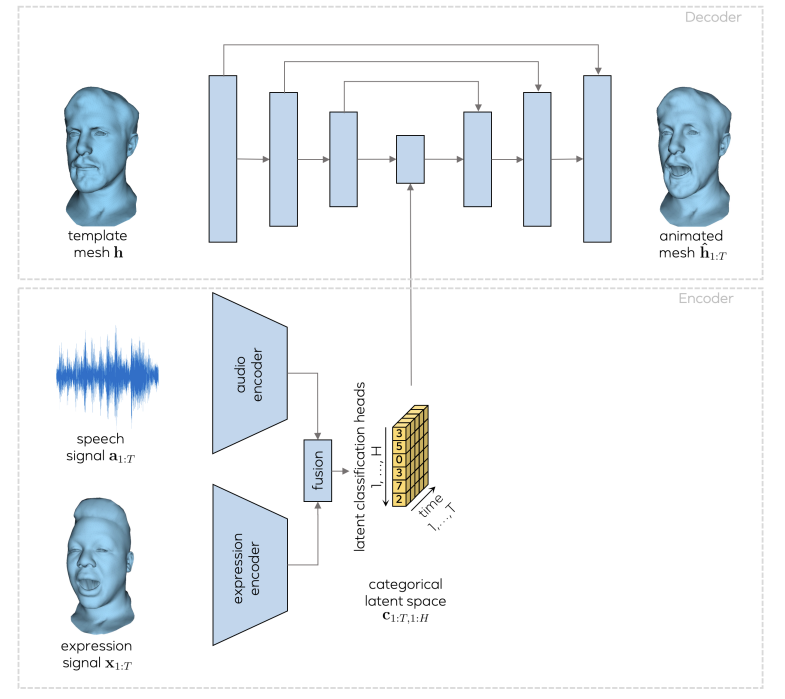
\includegraphics[width=7cm]{meshtalk_overview.png}
\caption{Meshtalk System Overview\ref{Richard2021-he} (Fig. 1)}
\end{figure}


\section{Assessing final manuscript length}
The Universal Manuscript Template is based on the Express journal layout and will provide an accurate length estimate for \emph{Optics Express}, \emph{Biomedical Optics Express},  \emph{Optical Materials Express}, and our newest title \emph{OSA Continuum}. \emph{Applied Optics}, JOSAA, JOSAB, \emph{Optics Letters}, \emph{Optica}, and \emph{Photonics Research} publish articles in a two-column layout. To estimate the final page count in a two-column layout, multiply the manuscript page count (in increments of 1/4 page) by 60\%. For example, 11.5 pages in the Universal Manuscript Template are roughly equivalent to 7 composed two-column pages. Note that the estimate is only an approximation, as treatment of figure sizing, equation display, and other aspects can vary greatly across manuscripts. Authors of Letters may use the legacy template for a more accurate length estimate.

\section{Figures, tables, and supplementary materials}

\subsection{Figures and tables}
Figures and tables should be placed in the body of the manuscript. Standard \LaTeX{} environments should be used to place tables and figures:
\begin{verbatm}
\begin{figure}[htbp]
\centering\includegraphics[width=7cm]{osafig1}
\caption{Sample caption (Fig. 2, \cite{Yelin:03}).}
\end{figure}
\end{verbatim}
%Ɗ(\rho)

\subsection{Supplementary materials in Optica Publishing Group journals}
Our journals allow authors to include supplementary materials as integral parts of a manuscript. Such materials are subject to peer-review procedures along with the rest of the paper and should be uploaded and described using our Prism manuscript system. Please refer to the \href{https://opg.optica.org/submit/style/supplementary_materials.cfm}{Author Guidelines for Supplementary Materials in Optica Publishing Group Journals} for more detailed instructions on labeling supplementary materials and your manuscript.

\textbf{Authors may also include Supplemental Documents} (PDF documents with expanded descriptions or methods) with the primary manuscript. At this time, supplemental PDF files are not accepted for partner titles, JOCN and \emph{Photonics Research}. To reference the supplementary document, the statement ``See Supplement 1 for supporting content.'' should appear at the bottom of the manuscript (above the References heading). 

\subsection{Sample Dataset Citation}

1. M. Partridge, "Spectra evolution during coating," figshare (2014), http://dx.doi.org/10.6084/m9.figshare.1004612.

\subsection{Sample Code Citation}

2. C. Rivers, "Epipy: Python tools for epidemiology," figshare (2014) [retrieved 13 May 2015], http://dx.doi.org/10.6084/m9.figshare.1005064.



\section{Mathematical and scientific notation}

\subsection{Displayed equations} Displayed equations should be centered.
Equation numbers should appear at the right-hand margin, in
parentheses:
\begin{equation}
Ɗ(\rho) =
 \frac{\gamma^2}{2} \; \sum_{k({\rm even}) = -\infty}^{\infty}
	\frac{(1 + k \tau)}{ \left[ (1 + k \tau)^2 + (\gamma  \rho)^2  \right]^{3/2} }.
\end{equation}

All equations should be numbered in the order in which they appear
and should be referenced  from within the main text as Eq. (1),
Eq. (2), and so on [or as inequality (1), etc., as appropriate].

\section{Backmatter}

Backmatter sections should be listed in the order Funding/Acknowledgment/Disclosures/Data Availability Statement/Supplemental Document section. An example of backmatter with each of these sections included is shown below.

\begin{backmatter}
\bmsection{Funding}
Content in the funding section will be generated entirely from details submitted to Prism. Authors may add placeholder text in the manuscript to assess length, but any text added to this section in the manuscript will be replaced during production and will display official funder names along with any grant numbers provided. If additional details about a funder are required, they may be added to the Acknowledgments, even if this duplicates information in the funding section. See the example below in Acknowledgements.

\bmsection{Acknowledgments}
Acknowledgments should be included at the end of the document. The section title should not follow the numbering scheme of the body of the paper. Additional information crediting individuals who contributed to the work being reported, clarifying who received funding from a particular source, or other information that does not fit the criteria for the funding block may also be included; for example, ``K. Flockhart thanks the National Science Foundation for help identifying collaborators for this work.'' 

\bmsection{Disclosures}
Disclosures should be listed in a separate nonnumbered section at the end of the manuscript. List the Disclosures codes identified on the \href{https://opg.optica.org/submit/review/data-availability-policy.cfm}{Conflict of Interest policy page}, as shown in the examples below:

\medskip

\noindent ABC: 123 Corporation (I,E,P), DEF: 456 Corporation (R,S). GHI: 789 Corporation (C).

\medskip

\noindent If there are no disclosures, then list ``The authors declare no conflicts of interest.''


\bmsection{Data Availability Statement}
A Data Availability Statement (DAS) will be required for all submissions beginning 1 March 2021. The DAS should be an unnumbered separate section titled ``Data Availability'' that
immediately follows the Disclosures section. See the \href{https://www.osapublishing.org/submit/review/data-availability-policy.cfm}{Data Availability Statement policy page} for more information.

OSA has identified four common (sometimes overlapping) situations that authors should use as guidance. These are provided as minimal models, and authors should feel free to
include any additional details that may be relevant.

\begin{enumerate}
\item When datasets are included as integral supplementary material in the paper, they must be declared (e.g., as "Dataset 1" following our current supplementary materials policy) and cited in the DAS, and should appear in the references.

\bmsection{Data availability} Data underlying the results presented in this paper are available in Dataset 1, Ref. [3].

\bigskip

\item When datasets are cited but not submitted as integral supplementary material, they must be cited in the DAS and should appear in the references.

\bmsection{Data availability} Data underlying the results presented in this paper are available in Ref. [3].

\bigskip

\item If the data generated or analyzed as part of the research are not publicly available, that should be stated. Authors are encouraged to explain why (e.g.~the data may be restricted for privacy reasons), and how the data might be obtained or accessed in the future.

\bmsection{Data availability} Data underlying the results presented in this paper are not publicly available at this time but may be obtained from the authors upon reasonable request.

\bigskip

\item If no data were generated or analyzed in the presented research, that should be stated.

\bmsection{Data availability} No data were generated or analyzed in the presented research.
\end{enumerate}


\bmsection{Supplemental document}
See Supplement 1 for supporting content. 

\end{backmatter}

\section{References}
\label{sec:refs}
Proper formatting of references is extremely important, not only for consistent appearance but also for accurate electronic tagging. Please follow the guidelines provided below on formatting, callouts, and use of Bib\TeX.

\subsection{Formatting reference items}
Each source must have its own reference number. Footnotes (notes at the bottom of text pages) are not used in our journals. References require all author names, full titles, and inclusive pagination. Examples of common reference types can be found in the  \href{https://www.osapublishing.org/submit/style/osa-styleguide.cfm} {style guide}.


The commands \verb+\begin{thebibliography}{}+ and \verb+\end{thebibliography}+ format the section according to standard style, showing the title {\bfseries References}.  Use the \verb+\bibitem{label}+ command to start each reference.

\subsection{Formatting reference citations}
References should be numbered consecutively in the order in which they are referenced in the body of the paper. Set reference callouts with standard \verb+\cite{}+ command or set manually inside square brackets [1].

To reference multiple articles at once, simply use a comma to separate the reference labels, e.g. \verb+\cite{Yelin:03,Masajada:13,Zhang:14}+, produces \cite{Yelin:03,Masajada:13,Zhang:14}.
%Using the \texttt{cite.sty} package will make these citations appear like so: [2--4].

\subsection{Bib\TeX}
\label{sec:bibtex}
Bib\TeX{} may be used to create a file containing the references, whose contents (i.e., contents of \texttt{.bbl} file) can then be pasted into the bibliography section of the \texttt{.tex} file. A Bib\TeX{} style file, \texttt{osajnl.bst}, is provided.

If your manuscript already contains a manually formatted \verb|\begin{thebibliography}|... \verb|\end{thebibliography}| list, then delete the \texttt{latexmkrc} file (if present) from your submission files. However you should ensure that your manually-formatted reference list adheres to style accurately.

\section{Conclusion}
After proofreading the manuscript, compress your .tex manuscript file and all figures (which should be in EPS or PDF format) in a ZIP, TAR or TAR-GZIP package. All files must be referenced at the root level (e.g., file \texttt{figure-1.eps}, not \texttt{/myfigs/figure-1.eps}). If there are supplementary materials, the associated files should not be included in your manuscript archive but be uploaded separately through the Prism interface.

%%%%%%%%%%%%%%%%%%%%%%% References %%%%%%%%%%%%%%%%%%%%%%%%%

Add references with BibTeX or manually.
\cite{Richard2021-he}


\end{document}
